\documentclass[../../main.tex]{subfiles}

\graphicspath{{../../image/}{../../figure/}}

\begin{document}

\section{Gauss 混合分布}\label{section:ch15-Gauss混合分布}

我们之前已经将 Gauss 混合分布描述为 Gauss 分量的简单线性叠加，目的是提供比单个 Gauss 分布更丰富的密度模型类别（参见\cref{subsection:ch03-Gauss混合}）。在本节中，将转向用离散潜变量的形式来描述 Gauss 混合分布。这将帮助我们更深入地理解这个重要分布，并有助于激励我们去探究 EM（Expectation--Maximization，最大期望）算法。

回想一下\eqref{align:ch03-Gauss混合}，Gauss 混合分布可以写成 Gauss 分量的线性叠加形式。

\begin{definition}[Gauss 混合分布]\label{definition:ch15-Gauss混合分布}
设 $K\geqslant1$，$\bm{\mu}_k\in\mathbb{R}^{D}$，$\bm{\Sigma}_k$ 为 $D\times D$ 正定对称矩阵，$k=1,\cdots,K$。称
\begin{align}
p(\bm{x})=\sum_{k=1}^{K}\pi_k\,\mathcal{N}(\bm{x}\,|\,\bm{\mu}_k,\bm{\Sigma}_k)
\label{align:ch15-gmm-marginal}
\end{align}
为 $K$ 个分量的 Gauss 混合分布（Gaussian mixture distribution，GMM），其中 $\mathcal{N}(\bm{x}\,|\,\bm{\mu}_k,\bm{\Sigma}_k)$ 称为第 $k$ 个\textbf{分量}，$\pi_k$ 称为第 $k$ 个\textbf{混合系数}。参数 $\{\pi_k\}$ 必须满足
\begin{align}
0\leqslant\pi_k\leqslant1
\label{align:ch15-pi-bounds}
\end{align}
和
\begin{align}
\sum_{k=1}^{K}\pi_k=1.
\label{align:ch15-pi-sum}
\end{align}
\end{definition}

% SUPPLEMENT: parent=definition:ch15-Gauss混合分布; kind=motivation; location=紧随其后的 remark（重构新增）
\begin{remark}（重构新增）
把若干 Gauss 密度加权相加，动机是让每个分量只负责一个“局部团块”，从而用简单的分量拼出多峰的复杂密度；\cref{section:ch15-K均值聚类}的 K 均值正是每个分量协方差都相同且趋于零时的极限情形（见\cref{subsection:ch15-em与kmeans}）。条件\eqref{align:ch15-pi-bounds}与\eqref{align:ch15-pi-sum}的作用各不相同：前者保证每一项都非负，从而 $p(\bm{x})\geqslant0$；后者保证 $\int p(\bm{x})\,\mathrm{d}\bm{x}=\sum_k\pi_k=1$，即 $p$ 是合法的概率密度。二者缺一不可——只去掉非负性，$\pi_k$ 为负时积分仍可能为 $1$，但 $p$ 在某些区域会取负值。各 $\bm{\Sigma}_k$ 的正定性保证 $\mathcal{N}(\bm{x}\,|\,\bm{\mu}_k,\bm{\Sigma}_k)$ 良定义且可归一化。注意分量个数 $K$ 不是由\eqref{align:ch15-gmm-marginal}决定的参数，而是模型结构的一部分；$K$ 越大模型越灵活，但参数个数 $K-1+K(D+D(D+1)/2)$ 也随之线性增长，且似然函数会出现\cref{proposition:ch15-似然奇异性}所述的奇异性。
\end{remark}

让我们引入一个 $K$ 维的二进制随机向量 $\bm{z}$，它采用 1-of-$K$ 表示形式，其中一个元素等于 $1$，其他所有元素等于 $0$。因此 $z_k$ 的值满足 $z_k\in\{0,1\}$ 以及 $\sum_k z_k=1$，并且根据哪个元素非零，向量 $\bm{z}$ 有 $K$ 种可能的状态。将联合分布 $p(\bm{x},\bm{z})$ 定义为边缘分布 $p(\bm{z})$ 和条件分布 $p(\bm{x}\,|\,\bm{z})$ 的形式。

\begin{definition}[1-of-$K$ 离散潜变量表示]\label{definition:ch15-离散潜变量}
设 $\bm{z}=(z_1,\cdots,z_K)^{\mathsf T}$ 满足 $z_k\in\{0,1\}$ 与 $\sum_{k=1}^{K}z_k=1$。关于 $\bm{z}$ 的边缘分布由混合系数 $\pi_k$ 指定，即
\begin{align*}
p(z_k=1)=\pi_k,
\end{align*}
其中参数 $\{\pi_k\}$ 满足\eqref{align:ch15-pi-bounds}与\eqref{align:ch15-pi-sum}。因为 $\bm{z}$ 使用 1-of-$K$ 表示形式，该分布也可以写成
\begin{align}
p(\bm{z})=\prod_{k=1}^{K}\pi_k^{z_k}.
\label{align:ch15-prior-factorized}
\end{align}
给定 $\bm{z}$ 的特定值时 $\bm{x}$ 的条件分布也是一个 Gauss 分布：
\begin{align*}
p(\bm{x}\,|\,z_k=1)=\mathcal{N}(\bm{x}\,|\,\bm{\mu}_k,\bm{\Sigma}_k),
\end{align*}
它可以写成
\begin{align}
p(\bm{x}\,|\,\bm{z})=\prod_{k=1}^{K}\mathcal{N}(\bm{x}\,|\,\bm{\mu}_k,\bm{\Sigma}_k)^{z_k}.
\label{align:ch15-conditional-x}
\end{align}
\end{definition}

% SUPPLEMENT: parent=definition:ch15-离散潜变量; kind=motivation; location=紧随其后的 remark（重构新增）
\begin{remark}（重构新增）
这个定义把“混合分布”改写成一个两层的生成过程：先按 $p(\bm{z})$ 抽一个状态（即选出分量），再按对应的 Gauss 密度抽 $\bm{x}$。定义中的两条乘积式\eqref{align:ch15-prior-factorized}与\eqref{align:ch15-conditional-x}是该表示能工作的关键：由于 $\bm{z}$ 是 1-of-$K$ 向量，$\prod_k\pi_k^{z_k}$ 中只有第 $k$ 个（$z_k=1$ 的那个）因子存活，值恰为 $\pi_k$，其余因子都是 $\pi_j^{0}=1$；同理\eqref{align:ch15-conditional-x}中只有第 $k$ 个 Gauss 因子存活。这样就把“按状态取分支”写成了统一的乘积形式，从而可以直接取对数、求和与求导。注意 $z_k\in\{0,1\}$ 与 $\sum_kz_k=1$ 是硬约束：$\bm{z}$ 的取值只有 $K$ 个，而不是 $2^{K}$ 个，这正是“离散潜变量”中“离散”的含义。
\end{remark}

联合分布由 $p(\bm{z})p(\bm{x}\,|\,\bm{z})$ 给出，它可以用\cref{figure:ch15-gmm-graph}中的图模型来描述（参见\cref{exercise:ch15-03}）。可以通过对所有可能的 $\bm{z}$ 的状态求和联合分布来获得 $\bm{x}$ 的边缘分布：
\begin{align}
p(\bm{x})=\sum_{\bm{z}}p(\bm{z})p(\bm{x}\,|\,\bm{z})=\sum_{k=1}^{K}\pi_k\mathcal{N}(\bm{x}\,|\,\bm{\mu}_k,\bm{\Sigma}_k),
\label{align:ch15-gmm-marginal-2}
\end{align}
其中我们利用了\eqref{align:ch15-prior-factorized}和\eqref{align:ch15-conditional-x}。因此，$\bm{x}$ 的边缘分布是形式为\eqref{align:ch15-gmm-marginal}的 Gauss 混合分布。如果我们有多个观测值 $\bm{x}_1,\cdots,\bm{x}_N$，那么因为边缘分布的形式是 $p(\bm{x})=\sum_{\bm{z}}p(\bm{x},\bm{z})$，所以每个观测到的数据点 $\bm{x}_n$ 都对应一个潜变量 $\bm{z}_n$。

\begin{figure}[htbp]
\centering
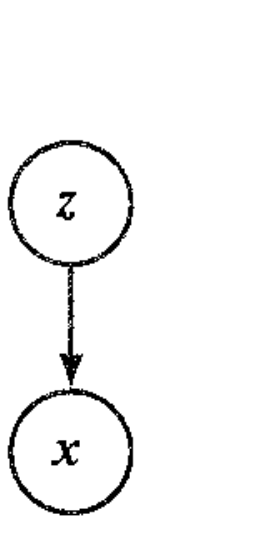
\includegraphics[width=0.085\textwidth]{ch15-fig15.4-latent-graph.png}
\caption{联合分布的图模型表示，其中联合分布以 $p(\bm{x},\bm{z})=p(\bm{z})p(\bm{x}\,|\,\bm{z})$ 的形式给出}
\label{figure:ch15-gmm-graph}
\end{figure}

\begin{proposition}[边缘化恢复混合分布]\label{proposition:ch15-边缘化}
设 $p(\bm{z})$ 由\eqref{align:ch15-prior-factorized}给出，$p(\bm{x}\,|\,\bm{z})$ 由\eqref{align:ch15-conditional-x}给出，则联合分布 $p(\bm{x},\bm{z})=p(\bm{z})p(\bm{x}\,|\,\bm{z})$ 关于 $\bm{z}$ 的边缘分布恰为\eqref{align:ch15-gmm-marginal}。
\end{proposition}
\begin{proof}
对 $\bm{z}$ 的所有 $K$ 种可能取值求和。由于 $\bm{z}$ 取遍 1-of-$K$ 向量，求和只有 $K$ 个非零项，且第 $k$ 项对应 $z_k=1$、其余 $z_j=0$。对这样的 $\bm{z}$，
\begin{align*}
p(\bm{z})=\prod_{j=1}^{K}\pi_j^{z_j}=\pi_k,\qquad
p(\bm{x}\,|\,\bm{z})=\prod_{j=1}^{K}\mathcal{N}(\bm{x}\,|\,\bm{\mu}_j,\bm{\Sigma}_j)^{z_j}=\mathcal{N}(\bm{x}\,|\,\bm{\mu}_k,\bm{\Sigma}_k).
\end{align*}
于是
\begin{align*}
p(\bm{x})=\sum_{\bm{z}}p(\bm{z})p(\bm{x}\,|\,\bm{z})=\sum_{k=1}^{K}\pi_k\mathcal{N}(\bm{x}\,|\,\bm{\mu}_k,\bm{\Sigma}_k),
\end{align*}
即\eqref{align:ch15-gmm-marginal}。
\end{proof}

% SUPPLEMENT: parent=proposition:ch15-边缘化; kind=motivation; location=紧随其后的 remark（重构新增）
\begin{remark}（重构新增）
这条命题说明了“引入潜变量没有改变模型”：$\bm{z}$ 只是把\eqref{align:ch15-gmm-marginal}中的求和换了一种说法，边缘分布仍然是同一个 Gauss 混合分布。它的价值在于把\textbf{求和}搬到了联合分布这一层，从而在完全数据情形下对数可以直接作用到每个分量（见\cref{subsection:ch15-Gauss混合em}）。证明只用到 $\bm{z}$ 的 1-of-$K$ 结构：求和项数等于 $K$ 而不是 $2^{K}$，这既保证了对 $\bm{z}$ 求和的可行性，也是后面 E 步骤只需计算 $K$ 个责任值的原因。若 $\bm{z}$ 的各分量独立（而非 1-of-$K$ 约束），边缘化将产生 $2^{K}$ 项，模型就不再是混合分布了。
\end{remark}

另一个起到重要作用的量是给定 $\bm{x}$ 时 $\bm{z}$ 的条件概率。我们使用 $\gamma(z_k)$ 来表示 $p(z_k=1\,|\,\bm{x})$，其值可以使用 Bayes 定理找到：
\begin{align}
\gamma(z_k)\equiv p(z_k=1\,|\,\bm{x})
&=\frac{p(z_k=1)p(\bm{x}\,|\,z_k=1)}{\sum_{j=1}^{K}p(z_j=1)p(\bm{x}\,|\,z_j=1)}\nonumber\\
&=\frac{\pi_k\mathcal{N}(\bm{x}\,|\,\bm{\mu}_k,\bm{\Sigma}_k)}{\sum_{j=1}^{K}\pi_j\mathcal{N}(\bm{x}\,|\,\bm{\mu}_j,\bm{\Sigma}_j)}.
\label{align:ch15-responsibility}
\end{align}

\begin{definition}[责任]\label{definition:ch15-责任}
称\eqref{align:ch15-responsibility}中的 $\gamma(z_k)=p(z_k=1\,|\,\bm{x})$ 为第 $k$ 个分量对观测值 $\bm{x}$ 的\textbf{责任}（responsibility）。
\end{definition}

% SUPPLEMENT: parent=definition:ch15-责任; kind=motivation; location=紧随其后的 remark（重构新增）
\begin{remark}（重构新增）
$\pi_k$ 可以视为 $z_k=1$ 的先验概率，$\gamma(z_k)$ 可以视为观测到 $\bm{x}$ 之后的相应后验概率。正如我们稍后将看到的，$\gamma(z_k)$ 也可以视为分量 $k$ 对“解释”观测值 $\bm{x}$ 所要承担的责任。从定义可以直接读出两条性质：$\gamma(z_k)\in[0,1]$ 且 $\sum_{k=1}^{K}\gamma(z_k)=1$，即责任是一个合法的“软分配”权重；这正是它与 K 均值中 $r_{nk}\in\{0,1\}$ 的硬分配的本质区别。责任依赖于 $\bm{x}$ 与全部分量参数的比较（分母对所有 $j$ 求和），因此它不是某个分量的“局部”属性；但当某个分量的密度远大于其他分量时，$\gamma(z_k)$ 会迅速趋近于 $1$，这正是\cref{subsection:ch15-em与kmeans}中 $\varepsilon\to0$ 极限下退化为硬分配的原因。名字“责任”的来历也在这里：$\gamma(z_k)$ 衡量的是“观测到 $\bm{x}$ 之后，把这一点归因于第 $k$ 个分量的可信程度”。
\end{remark}

参见\cref{subsection:ch14-祖先采样}，我们可以使用祖先采样（ancestral sampling）生成随机样本，这些样本按照 Gauss 混合模型分布。为此，我们首先从边缘分布 $p(\bm{z})$ 中生成一个 $\bm{z}$ 的值，记为 $\hat{\bm{z}}$，然后从条件分布 $p(\bm{x}\,|\,\hat{\bm{z}})$ 中生成一个 $\bm{x}$ 的值。我们可以通过在对应的 $\bm{x}$ 值处绘制点，然后根据 $\bm{z}$ 的值（即生成这些点的 Gauss 分量）对点进行着色来描绘联合分布 $p(\bm{x},\bm{z})$ 中的样本，如\cref{figure:ch15-responsibility}(a) 所示。类似地，边缘分布 $p(\bm{x})$ 中的样本是通过选取联合分布中的样本并忽略 $\bm{z}$ 的值获得的。这些样本如\cref{figure:ch15-responsibility}(b) 所示，仅依据 $\bm{x}$ 值绘制出点而不带任何颜色标签。

\begin{figure}[htbp]
\centering
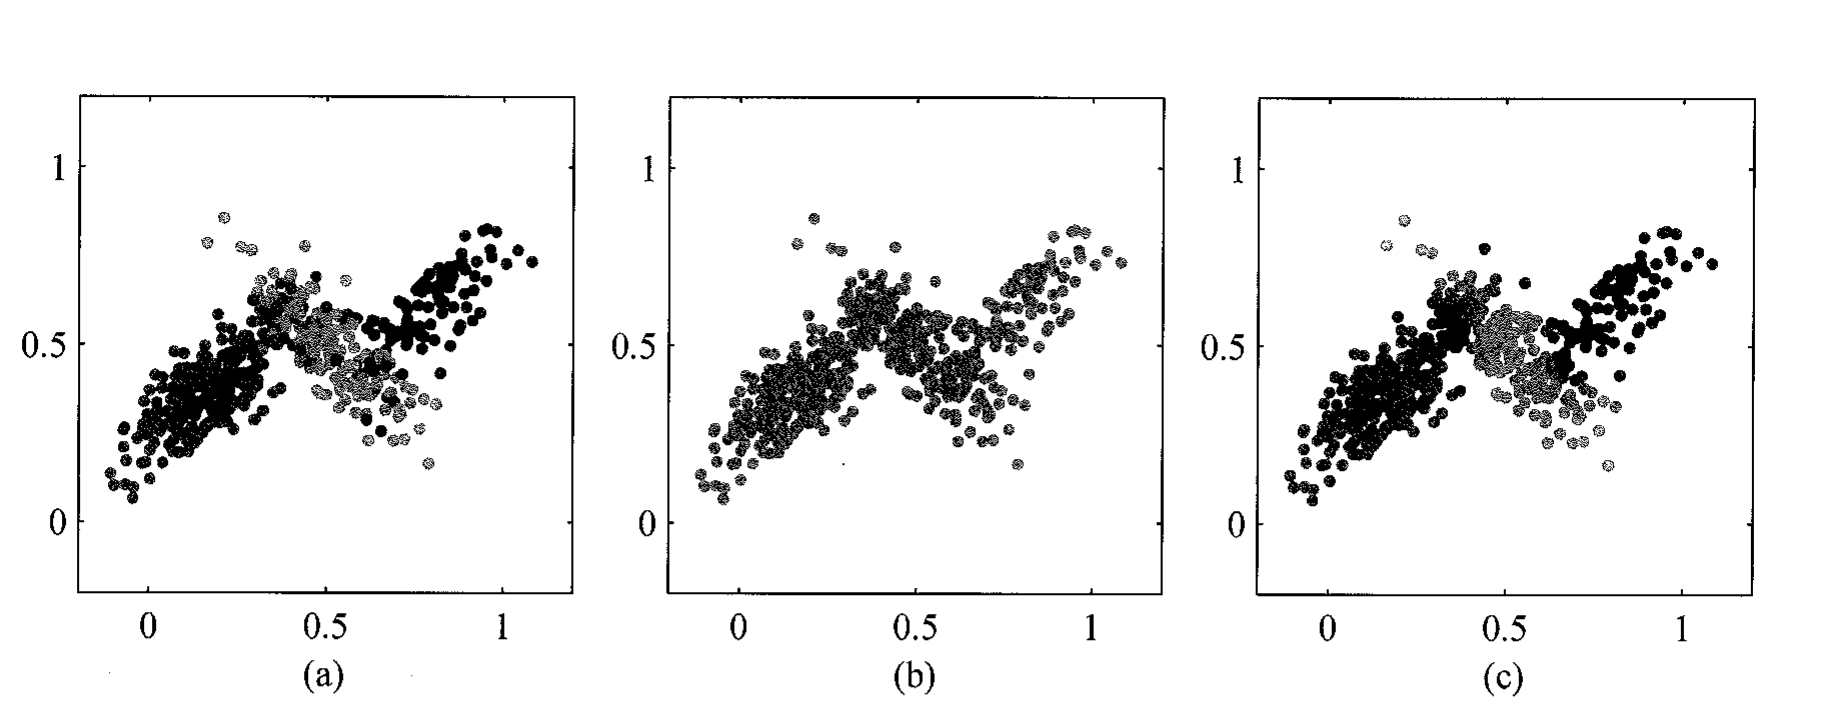
\includegraphics[width=0.95\textwidth]{ch15-fig15.5-responsibility.png}
\caption{从\cref{figure:ch03-混合等值线}所示的三个 Gauss 混合分布中抽取 500 个数据点的示例。(a)~来自联合分布 $p(\bm{z})p(\bm{x}\,|\,\bm{z})$ 的样本，其中 $\bm{z}$ 的三种状态分别对应于混合的三个分量，分别用红色、绿色和蓝色表示。(b)~来自边缘分布 $p(\bm{x})$ 的相应样本，该边缘分布是通过简单地忽略 $\bm{z}$ 的值并仅绘制 $\bm{x}$ 的值获得的，数据集在 (a) 中被认为是完整的，而在 (b) 中被认为是不完整的（参见\cref{section:ch15-em算法}）。(c)~相同的样本，其中颜色代表与数据点 $\bm{x}_n$ 相关的责任 $\gamma(z_{nk})$，当 $k$ 取值分别为 $1,2,3$ 时，可通过调配红色、蓝色和绿色比例来绘制相应的点来获得}
\label{figure:ch15-responsibility}
\end{figure}

我们还可以使用这个合成的数据集来说明“责任”，即评估每个数据点关于生成此数据集的 Gauss 混合分布中每个分量的后验概率。特别地，我们可以使用红色、蓝色和绿色墨水的比例来表示与数据点 $\bm{x}_n$ 相关的责任 $\gamma(z_{nk})$ 的值。每个点所用的这三种墨水的比例由 $\gamma(z_{nk})$ 给出，$k=1,2,3$，如\cref{figure:ch15-responsibility}(c) 所示。例如，一个 $\gamma(z_{n1})=1$ 的数据点将染成红色，而一个 $\gamma(z_{n2})=\gamma(z_{n3})=0.5$ 的数据点将以等比例的蓝色和绿色染色，因此呈现为青色。而在\cref{figure:ch15-responsibility}(a) 中，将数据点标记成什么颜色依据的是它们实际所属的分量。

我们找到了一个涉及显式潜变量的 Gauss 混合分布的等效表示，其中联合分布以图模型的形式给出。这么做的收益看起来并不大。然而，现在我们已经能够用联合分布 $p(\bm{x},\bm{z})=p(\bm{z})p(\bm{x}\,|\,\bm{z})$ 代替边缘分布 $p(\bm{x})$ 工作，这将带来显著的简化（特别是在引入 EM 算法时）。

\subsection{似然函数}\label{subsection:ch15-似然函数}

假设我们有一组观测数据 $\{\bm{x}_1,\cdots,\bm{x}_N\}$，我们希望使用 Gauss 混合模型来对这些数据进行建模。我们可以将这个数据集表示为一个 $N\times D$ 的矩阵 $\bm{X}$，其中第 $n$ 行由 $\bm{x}_n^{\mathsf T}$ 给出。

由\eqref{align:ch15-gmm-marginal}可知，似然函数的对数由下式给出：
\begin{align}
\ln p(\bm{X}\,|\,\bm{\pi},\bm{\mu},\bm{\Sigma})=\sum_{n=1}^{N}\ln\!\left\{\sum_{k=1}^{K}\pi_k\mathcal{N}(\bm{x}_n\,|\,\bm{\mu}_k,\bm{\Sigma}_k)\right\}.
\label{align:ch15-gmm-nll}
\end{align}

最大化这个对数似然函数比针对单个 Gauss 分布更复杂。难点在于\eqref{align:ch15-gmm-nll}中的对数内部的求和项会导致对数不再直接作用于 Gauss 分布。如果将对数似然函数关于模型参数的导数设为零，我们将不再获得闭合解，这一点我们很快就会看到。

在讨论如何最大化这个函数之前，值得强调的是，在应用到 Gauss 混合模型时，最大似然框架存在一个显著的问题，就是有奇异性。为了简单起见，考虑一个 Gauss 混合模型，其组成部分的协方差矩阵由 $\bm{\Sigma}_k=\sigma_k^2\bm{I}$ 给出，其中 $\bm{I}$ 是单位矩阵，但所得结论对于一般的协方差矩阵也是成立的。假设该 Gauss 混合模型的一个分量，比如第 $j$ 个分量，其均值 $\bm{\mu}_j$ 恰好等于某个数据点，即 $\bm{\mu}_j=\bm{x}_n$，则这个数据点将在似然函数中贡献一个如下形式的项：
\begin{align}
\mathcal{N}\big(\bm{x}_n\,|\,\bm{x}_n,\sigma_j^2\bm{I}\big)=\frac{1}{(2\pi)^{1/2}}\frac{1}{\sigma_j}.
\label{align:ch15-singularity}
\end{align}

\begin{remark}（重构新增：原文问题说明）
\eqref{align:ch15-singularity}印出的是\textbf{一元}情形（$D=1$）的取值：$D=1$ 时 $\mathcal{N}(x\,|\,x,\sigma_j^2)=(2\pi\sigma_j^2)^{-1/2}=\frac{1}{(2\pi)^{1/2}}\frac{1}{\sigma_j}$，正是右端的形状。但同一式左端写的是向量 $\bm{x}_n$ 与矩阵 $\bm{I}$，按此记号应为 $D$ 元密度
\begin{align*}
\mathcal{N}\big(\bm{x}_n\,|\,\bm{x}_n,\sigma_j^2\bm{I}\big)=\frac{1}{(2\pi\sigma_j^2)^{D/2}},
\end{align*}
它在 $\sigma_j\to0$ 时以 $\sigma_j^{-D}$ 的速度发散，比一元情形更快。两种读法在“$\sigma_j\to0$ 时趋于无穷”这一定性结论上完全一致，下文与\cref{proposition:ch15-似然奇异性}的论证对一般 $D$ 成立。这里照译原式，并指出右端应按 $D=1$ 理解，引用时请以 $D$ 元形式为准。
\end{remark}

考虑极限 $\sigma_j\rightarrow0$，我们会看到该项趋向于无穷大，所以对数似然函数也将趋向于无穷大。由此可见，最大化对数似然函数并不是一个良定义的问题，因为这种奇异性总是存在的，并且每当一个 Gauss 分量“坍缩”到一个特定的数据点时就会发生。

\begin{proposition}[似然函数的奇异性]\label{proposition:ch15-似然奇异性}
设 $K\geqslant1$，$\pi_j>0$，且数据集中至少含有一个点 $\bm{x}_n$。则对数似然\eqref{align:ch15-gmm-nll}在参数空间上没有上界：对任意 $M>0$，都存在参数使得 $\ln p(\bm{X}\,|\,\bm{\pi},\bm{\mu},\bm{\Sigma})>M$。
\end{proposition}
\begin{proof}
固定 $n$ 与分量 $j$，取 $\bm{\mu}_j=\bm{x}_n$、$\bm{\Sigma}_j=\sigma_j^2\bm{I}$，其余分量任意固定。由于每一项 $\pi_k\mathcal{N}(\cdot)\geqslant0$，有
\begin{align*}
p(\bm{x}_n\,|\,\bm{\pi},\bm{\mu},\bm{\Sigma})
\geqslant\pi_j\,\mathcal{N}\big(\bm{x}_n\,|\,\bm{x}_n,\sigma_j^2\bm{I}\big)
=\frac{\pi_j}{(2\pi\sigma_j^2)^{D/2}}.
\end{align*}
当 $\sigma_j\to0^{+}$ 时右端趋于 $+\infty$，故 $p(\bm{x}_n\,|\,\cdot)\to+\infty$；又对数似然是 $N$ 项之和，其中第 $n$ 项为 $\ln p(\bm{x}_n\,|\,\cdot)$，而其余各项非负项的对数可能为负但有限，于是
\begin{align*}
\ln p(\bm{X}\,|\,\bm{\pi},\bm{\mu},\bm{\Sigma})\geqslant\ln p(\bm{x}_n\,|\,\bm{\pi},\bm{\mu},\bm{\Sigma})\longrightarrow+\infty.
\end{align*}
因此对任意 $M$ 都可取 $\sigma_j$ 足够小使对数似然超过 $M$，即无上界。
\end{proof}

% SUPPLEMENT: parent=proposition:ch15-似然奇异性; kind=motivation; location=紧随其后的 remark（重构新增）
\begin{remark}（重构新增）
这条命题说明“最大似然在 Gauss 混合模型中不是一个良定义的问题”：不是解不存在，而是目标函数没有上界，所谓“最大值”根本不存在（$\sup=+\infty$）。奇异性只要求某一个分量的均值精确落在某个数据点上、同时其协方差退化到零，因此它在参数空间中是一个低维但\textbf{稠密可达}的“坏集”：只要允许 $\bm{\Sigma}_k$ 任意小，优化过程就可能被吸引过去。条件“$\pi_j>0$”不可省——若某个混合系数严格为零，该分量对密度没有贡献，也就不会产生这个奇异项。对一般的（非各向同性）协方差矩阵，证明完全相同，只需把 $\sigma_j^2\bm{I}$ 换成一个行列式趋于零的正定矩阵，此时密度按 $\lvert\bm{\Sigma}_j\rvert^{-1/2}$ 发散。这一现象是最大似然过拟合的典型例子，处理办法见下文的启发式重置与参数先验（\cref{subsection:ch15-参数先验}）。
\end{remark}

这种奇异性提供了一个最大似然方法中可能出现过拟合的例子。当把最大似然方法应用到 Gauss 混合模型时，我们必须采取措施以避免找到这样的病态（pathological）解，比如转而寻求似然函数的局部最大值，这些局部最大值通常表现良好。我们可以试图通过使用适当的启发式方法来避免奇异性，例如检测到 Gauss 分量在坍缩时将其均值重置为随机选择的值，同时将其协方差重置为某个较大值，然后继续优化。通过添加一个对应于参数先验分布的正则化项到对数似然函数中，也可以避免奇异性（参见\cref{subsection:ch15-参数先验}）。

\begin{figure}[htbp]
\centering
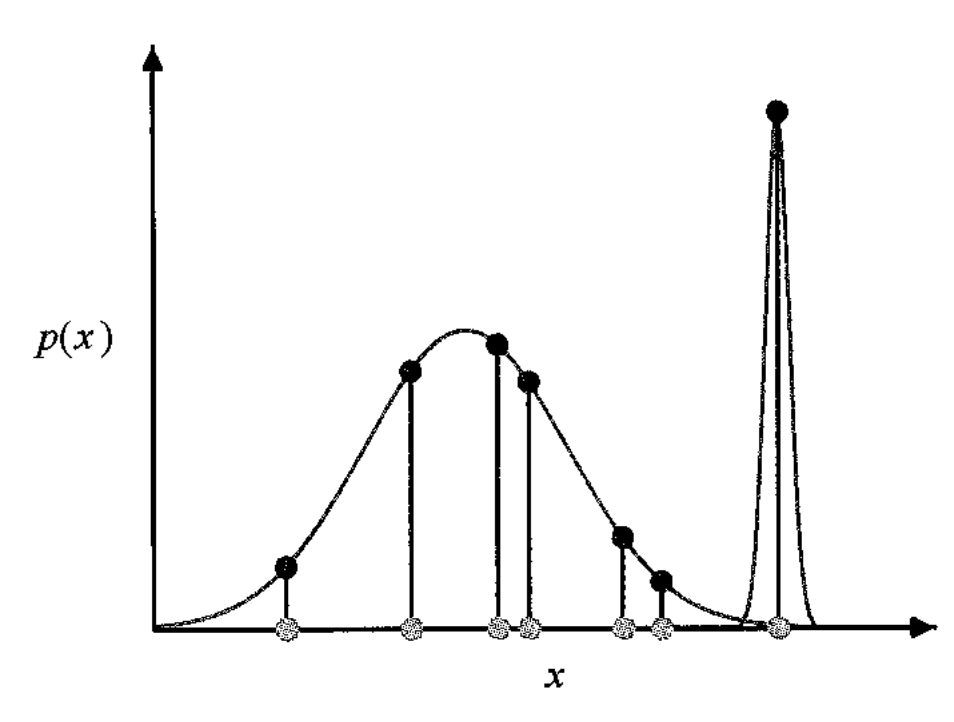
\includegraphics[width=0.3\textwidth]{ch15-fig15.6-singularity.png}
\caption{在 Gauss 混合模型中，似然函数中的奇异点是如何出现的。请和\cref{figure:ch02-似然函数}中显示的没有奇异点的情况进行比较}
\label{figure:ch15-singularity}
\end{figure}

在寻找最大似然解时还有一个问题，因为对于任何给定的最大似然解，一个包含 $K$ 个组分的 Gauss 混合模型将有总共 $K!$ 个等效解，对应于将 $K$ 组参数分配给 $K$ 个组分的 $K!$ 种方式。换句话说，对于参数值空间中的任何给定（非退化）点，都会存在额外的 $K!-1$ 个点。所有这些点都将产生完全相同的分布。这个问题称为可识别性（identifiability）问题（Casella and Berger, 2002），当我们希望解释模型发现的参数值时，这是一个重要问题。当我们讨论具有连续潜变量的模型（参见\cref{chapter:ch16-连续潜变量}）时，可识别性问题也会出现。然而，当我们寻找一个好的密度模型时，这个问题无关紧要，因为任何等效解都和其他解一样好。

\begin{proposition}[交换对称性导致的 $K!$ 个等价解]\label{proposition:ch15-交换对称性}
设 $\bm{\theta}=(\pi_1,\cdots,\pi_K,\bm{\mu}_1,\cdots,\bm{\mu}_K,\bm{\Sigma}_1,\cdots,\bm{\Sigma}_K)$ 给出\eqref{align:ch15-gmm-marginal}的一个参数组，且各分量互不相同（非退化）。对 $\{1,\cdots,K\}$ 的任一置换 $\sigma$，令 $\pi'_k=\pi_{\sigma(k)}$、$\bm{\mu}'_k=\bm{\mu}_{\sigma(k)}$、$\bm{\Sigma}'_k=\bm{\Sigma}_{\sigma(k)}$，则 $\bm{\theta}'$ 与 $\bm{\theta}$ 给出同一个密度。不同的置换给出不同的参数组，因此等价参数组恰有 $K!$ 个。
\end{proposition}
\begin{proof}
对任意 $\bm{x}$，
\begin{align*}
\sum_{k=1}^{K}\pi'_k\,\mathcal{N}(\bm{x}\,|\,\bm{\mu}'_k,\bm{\Sigma}'_k)
=\sum_{k=1}^{K}\pi_{\sigma(k)}\,\mathcal{N}(\bm{x}\,|\,\bm{\mu}_{\sigma(k)},\bm{\Sigma}_{\sigma(k)})
=\sum_{j=1}^{K}\pi_j\,\mathcal{N}(\bm{x}\,|\,\bm{\mu}_j,\bm{\Sigma}_j),
\end{align*}
这是因为 $\sigma$ 只是把求和指标 $\{1,\cdots,K\}$ 重新排列了一遍（令 $j=\sigma(k)$）。故两参数组给出同一密度。

再证不同的置换给出不同的参数组。置换群有 $K!$ 个元素；若 $\sigma\neq\sigma'$，则存在 $k$ 使 $\sigma(k)\neq\sigma'(k)$。若两参数组相同，则 $\pi_{\sigma(k)}=\pi_{\sigma'(k)}$、$\bm{\mu}_{\sigma(k)}=\bm{\mu}_{\sigma'(k)}$、$\bm{\Sigma}_{\sigma(k)}=\bm{\Sigma}_{\sigma'(k)}$；由非退化性（各分量互不相同，故分量由其参数三元组唯一标识），这迫使 $\sigma(k)=\sigma'(k)$，矛盾。因此这 $K!$ 个参数组两两不同。
\end{proof}

% SUPPLEMENT: parent=proposition:ch15-交换对称性; kind=motivation; location=紧随其后的 remark（重构新增）
\begin{remark}（重构新增）
这条命题是“可识别性”讨论的核心：模型作为\textbf{密度}是可识别的（不同分量组合给出不同密度，在非退化点处），但作为\textbf{参数化}不可识别（同一个密度对应 $K!$ 个参数组）。$K!$ 来自对称群而非参数的连续自由度，所以它不是“近似解”而是\textbf{精确}的等价：两参数组给出的 $p(\bm{x})$ 处处相等。后果有两点。其一，任何以参数为对象的推断（例如“第 3 个分量对应哪个簇”）都必须先固定一个规范次序或事后重新排序，否则结论没有意义。其二，$K!$ 个等价解使似然函数的驻点成倍出现，但它们的最优值相同，故对“找好的密度模型”这一目标没有影响；这也解释了为什么 EM 算法可以收敛到其中任意一个。非退化条件不可省：若两个分量参数完全相同，则交换它们得到的是同一个参数组，$K!$ 的计数需要按重数修正。
\end{remark}

\subsection{最大似然}\label{subsection:ch15-最大似然}

在为含有隐变量的模型寻找最大似然解的探索中，EM 算法是一种优雅而强大的方法（Dempster, Laird and Rubin, 1977; McLachlan and Krishnan, 1997）。在本章中，我们将先后给出三种不同的 EM 算法推导，每一种都比前一种更加通用。下面让我们在 Gauss 混合模型的背景下以相对非正式的方式开始。首先需要强调的是，EM 算法具有广泛的适用性，它的底层概念我们将在本书涉及的多个模型中遇到。

我们选择从写下似然函数最大值处必须满足的条件开始。将\eqref{align:ch15-gmm-nll}中的 $\ln p(\bm{X}\,|\,\bm{\pi},\bm{\mu},\bm{\Sigma})$ 关于 Gauss 分量均值 $\bm{\mu}_k$ 的导数设为零，便可得到
\begin{align}
0=\sum_{n=1}^{N}\underbrace{\frac{\pi_k\mathcal{N}(\bm{x}_n\,|\,\bm{\mu}_k,\bm{\Sigma}_k)}{\sum_j\pi_j\mathcal{N}(\bm{x}_n\,|\,\bm{\mu}_j,\bm{\Sigma}_j)}}_{\gamma(z_{nk})}\bm{\Sigma}_k^{-1}(\bm{x}_n-\bm{\mu}_k),
\label{align:ch15-mu-deriv}
\end{align}
其中我们利用了 Gauss 分布的形式\eqref{align:ch03-多元Gauss}。注意，后验概率或责任 $\gamma(z_{nk})$ 由\eqref{align:ch15-responsibility}给出，因而自然地出现在公式的右侧。乘以 $\bm{\Sigma}_k$（我们假设它是非奇异的）并重新排列后，便可得到
\begin{align}
\bm{\mu}_k=\frac{1}{N_k}\sum_{n=1}^{N}\gamma(z_{nk})\,\bm{x}_n,
\label{align:ch15-mu-update}
\end{align}
其中我们定义了
\begin{align}
N_k=\sum_{n=1}^{N}\gamma(z_{nk}).
\label{align:ch15-effective-n}
\end{align}

可以将 $N_k$ 解释为分配给聚类 $k$ 的有效点数。仔细观察这个解的形式，可以看到，第 $k$ 个 Gauss 分量的均值 $\bm{\mu}_k$ 是通过对数据集中的所有点进行加权平均得到的。在这个加权因子中，数据点 $\bm{x}_n$ 的权重是由后验概率 $\gamma(z_{nk})$ 给出的，即第 $k$ 个 Gauss 分量负责生成 $\bm{x}_n$ 的概率。

如果将 $\ln p(\bm{X}\,|\,\bm{\pi},\bm{\mu},\bm{\Sigma})$ 关于 $\bm{\Sigma}_k$ 的导数设为零并遵循类似的推理线索，利用单个 Gauss 分布的最大似然解的结果（参见\cref{subsection:ch03-最大似然}），便可得到
\begin{align}
\bm{\Sigma}_k=\frac{1}{N_k}\sum_{n=1}^{N}\gamma(z_{nk})(\bm{x}_n-\bm{\mu}_k)(\bm{x}_n-\bm{\mu}_k)^{\mathsf T}.
\label{align:ch15-sigma-update}
\end{align}
这与用单个 Gauss 分布拟合数据集的对应结果形式相同，但每个数据点都由相应的后验概率加权，并且分母由与相应分量相关联的有效点数给出。

最后，我们调整混合系数 $\pi_k$ 的值，目的是最大化对数似然函数 $\ln p(\bm{X}\,|\,\bm{\pi},\bm{\mu},\bm{\Sigma})$。此处我们必须考虑一个约束［\eqref{align:ch15-pi-sum}］，该约束要求混合系数的和为 $1$。这可以通过使用 Lagrange 乘子 $\lambda$ 并最大化以下量来实现：
\begin{align}
\ln p(\bm{X}\,|\,\bm{\pi},\bm{\mu},\bm{\Sigma})+\lambda\!\left(\sum_{k=1}^{K}\pi_k-1\right).
\label{align:ch15-lagrangian}
\end{align}
这样便可得到
\begin{align}
0=\sum_{n=1}^{N}\frac{\mathcal{N}(\bm{x}_n\,|\,\bm{\mu}_k,\bm{\Sigma}_k)}{\sum_j\pi_j\mathcal{N}(\bm{x}_n\,|\,\bm{\mu}_j,\bm{\Sigma}_j)}+\lambda.
\label{align:ch15-pi-deriv}
\end{align}

可以看到“责任”再次出现了。如果对\eqref{align:ch15-pi-deriv}的两边乘以 $\pi_k$ 并利用\eqref{align:ch15-pi-sum}对 $k$ 进行求和，就会发现 $\lambda=-N$。消除 $\lambda$ 并重新排列后，便可得到
\begin{align}
\pi_k=\frac{N_k}{N}.
\label{align:ch15-pi-update}
\end{align}

因此，第 $k$ 个 Gauss 分量的混合系数由该分量对解释数据点所要承担的平均责任给出。

\begin{proposition}[Gauss 混合模型的最大似然方程]\label{proposition:ch15-GMM最大似然}
设 $N_k=\sum_n\gamma(z_{nk})>0$，$\bm{\Sigma}_k$ 非奇异。则对数似然\eqref{align:ch15-gmm-nll}的任一驻点 $(\bm{\pi},\bm{\mu},\bm{\Sigma})$ 满足\eqref{align:ch15-mu-update}、\eqref{align:ch15-sigma-update}与\eqref{align:ch15-pi-update}，其中 $\gamma(z_{nk})$ 由\eqref{align:ch15-responsibility}定义。
\end{proposition}
\begin{proof}
\textbf{（关于 $\bm{\mu}_k$）}记 $p_n=\sum_j\pi_j\mathcal{N}(\bm{x}_n\,|\,\bm{\mu}_j,\bm{\Sigma}_j)$。由 $\partial\ln p_n/\partial\bm{\mu}_k=\pi_k\mathcal{N}(\bm{x}_n\,|\,\bm{\mu}_k,\bm{\Sigma}_k)\cdot\big(-\bm{\Sigma}_k^{-1}(\bm{x}_n-\bm{\mu}_k)\big)/p_n$，并注意 $\pi_k\mathcal{N}(\bm{x}_n\,|\,\bm{\mu}_k,\bm{\Sigma}_k)/p_n=\gamma(z_{nk})$，得
\begin{align*}
\frac{\partial\ln p(\bm{X}\,|\,\cdot)}{\partial\bm{\mu}_k}
=-\sum_{n=1}^{N}\gamma(z_{nk})\,\bm{\Sigma}_k^{-1}(\bm{x}_n-\bm{\mu}_k).
\end{align*}
置零并左乘 $\bm{\Sigma}_k$ 得 $\sum_n\gamma(z_{nk})(\bm{x}_n-\bm{\mu}_k)=0$，即\eqref{align:ch15-mu-deriv}，从而 $\bm{\mu}_k=N_k^{-1}\sum_n\gamma(z_{nk})\bm{x}_n$。

\textbf{（关于 $\bm{\Sigma}_k$）}由 $\partial\ln p_n/\partial\bm{\Sigma}_k=\gamma(z_{nk})\,\partial\ln\mathcal{N}(\bm{x}_n\,|\,\bm{\mu}_k,\bm{\Sigma}_k)/\partial\bm{\Sigma}_k$ 以及单个 Gauss 密度的矩阵导数
\begin{align*}
\frac{\partial}{\partial\bm{\Sigma}_k}\ln\mathcal{N}(\bm{x}_n\,|\,\bm{\mu}_k,\bm{\Sigma}_k)
=\frac{1}{2}\bm{\Sigma}_k^{-1}-\frac{1}{2}\bm{\Sigma}_k^{-1}(\bm{x}_n-\bm{\mu}_k)(\bm{x}_n-\bm{\mu}_k)^{\mathsf T}\bm{\Sigma}_k^{-1},
\end{align*}
置零得
\begin{align*}
\frac{1}{2}\bm{\Sigma}_k^{-1}\sum_{n=1}^{N}\gamma(z_{nk})
=\frac{1}{2}\bm{\Sigma}_k^{-1}\left[\sum_{n=1}^{N}\gamma(z_{nk})(\bm{x}_n-\bm{\mu}_k)(\bm{x}_n-\bm{\mu}_k)^{\mathsf T}\right]\bm{\Sigma}_k^{-1}.
\end{align*}
左乘 $\bm{\Sigma}_k$、右乘 $\bm{\Sigma}_k$，并用 $N_k=\sum_n\gamma(z_{nk})$，即得\eqref{align:ch15-sigma-update}。这与单 Gauss 最大似然协方差（\cref{proposition:ch03-Gauss最大似然}）的推导完全平行，区别只在于每个数据点带着权重 $\gamma(z_{nk})$。

\textbf{（关于 $\bm{\pi}_k$）}在约束\eqref{align:ch15-pi-sum}下引入 Lagrange 乘子，得\eqref{align:ch15-lagrangian}。对 $\pi_k$ 求偏导并置零：
\begin{align*}
0=\sum_{n=1}^{N}\frac{\mathcal{N}(\bm{x}_n\,|\,\bm{\mu}_k,\bm{\Sigma}_k)}{p_n}+\lambda,
\end{align*}
即\eqref{align:ch15-pi-deriv}。两边乘 $\pi_k$，注意 $\pi_k\mathcal{N}(\bm{x}_n\,|\,\bm{\mu}_k,\bm{\Sigma}_k)/p_n=\gamma(z_{nk})$，得 $\sum_n\gamma(z_{nk})+\lambda\pi_k=0$。对 $k$ 求和并用 $\sum_k\pi_k=1$ 与 $\sum_k\gamma(z_{nk})=1$：
\begin{align*}
\sum_{k=1}^{K}\sum_{n=1}^{N}\gamma(z_{nk})+\lambda\sum_{k=1}^{K}\pi_k=N+\lambda=0,
\end{align*}
故 $\lambda=-N$。代回得 $\pi_k=N_k/N$，即\eqref{align:ch15-pi-update}。
\end{proof}

% SUPPLEMENT: parent=proposition:ch15-GMM最大似然; kind=motivation; location=紧随其后的 remark（重构新增）
\begin{remark}（重构新增）
这条命题给出了 EM 算法在 GMM 上的 M 步骤的全部内容，但要注意它是一个\textbf{隐式}方程组：右端的 $\gamma(z_{nk})$ 通过\eqref{align:ch15-responsibility}依赖于 $\bm{\mu}_k,\bm{\Sigma}_k,\bm{\pi}_k$ 本身，所以\eqref{align:ch15-mu-update}、\eqref{align:ch15-sigma-update}、\eqref{align:ch15-pi-update}并不是参数的闭合解，而是一组“若把责任看作已知量则成立”的方程。这正是 EM 的出发点：把责任当作缺失数据代入，方程就变成显式的。$N_k$ 的解释是“有效点数”，它不必是整数；当责任退化为 $0/1$ 时 $N_k$ 就是第 $k$ 个聚类中数据点的个数，于是\eqref{align:ch15-mu-update}退化为 K 均值的均值更新\eqref{align:ch15-kmeans-mu}。推导中用到的两个条件——$\bm{\Sigma}_k$ 非奇异（否则 $\bm{\Sigma}_k^{-1}$ 无定义）与 $N_k>0$（否则均值无定义）——在数值实现中都要显式检查：前者由\cref{proposition:ch15-似然奇异性}说明可能失效，后者意味着某个分量“没有分到任何质量”，此时应删除该分量或重新初始化。
\end{remark}

请注意，\eqref{align:ch15-mu-update}、\eqref{align:ch15-sigma-update}和\eqref{align:ch15-pi-update}并不构成 Gauss 混合模型参数的闭合解，因为责任 $\gamma(z_{nk})$ 通过\eqref{align:ch15-responsibility}以复杂的方式依赖于这些参数。然而，这些结果确实提出了一种简单的迭代方案来寻找最大似然问题的解。正如我们将看到的，对于 Gauss 混合模型的特定情况，这实际上是 EM 算法的一个实例。我们首先选择均值、协方差和混合系数的一些初始值，然后交替进行以下两个步骤——期望步骤（E 步骤）和最大化步骤（M 步骤）。在 E 步骤中，我们使用参数的当前值来估计后验概率或责任，其由\eqref{align:ch15-responsibility}给出。然后在 M 步骤中使用这些概率重新估计均值、协方差和混合系数，它们分别由\eqref{align:ch15-mu-update}、\eqref{align:ch15-sigma-update}和\eqref{align:ch15-pi-update}给出。请注意，当决定这样做时，我们首先使用\eqref{align:ch15-mu-update}计算新的均值，然后使用这些新值通过\eqref{align:ch15-sigma-update}找到协方差，其与单个 Gauss 分布的相应结果一致。我们将证明每次进行 E 步骤之后，紧跟着进行的 M 步骤导致的参数更新都会增大对数似然函数的值。在实践中，当对数似然函数的值的变化，或者说参数的值的变化低于某个阈值时，算法就被认为已经收敛。

下面我们用重缩放的老忠实喷泉数据集来说明应用于 Gauss 混合模型的 EM 算法，如\cref{figure:ch15-em-iter}所示。这里使用了两个 Gauss 分量，其聚类中心使用与\cref{figure:ch15-kmeans}中 K 均值算法相同的值进行初始化，协方差矩阵则初始化为与单位矩阵成比例。\cref{figure:ch15-em-iter}(a) 显示了绿色的数据点以及 Gauss 混合模型的初始配置，其中两个 Gauss 分量的一倍标准差轮廓线分别显示为蓝色和红色圆圈。\cref{figure:ch15-em-iter}(b) 显示了 E 步骤的初始结果，其中每个数据点使用与从蓝色分量生成的后验概率相等的蓝色墨水比例绘制，并且绘制时还使用了由红色分量生成的后验概率所给出的相应比例的红色墨水。因此，那些属于两个聚类的概率大致相等的点呈现为紫色。第一次进行 M 步骤后的情况如\cref{figure:ch15-em-iter}(c) 所示，蓝色分量的均值已移动到由每个数据点属于蓝色聚类的概率加权的数据集的均值上。换句话说，其已经移动到了蓝色墨水的中心位置。同样，蓝色分量的协方差已设定为蓝色墨水的协方差。对于红色分量也有类似的结果。\cref{figure:ch15-em-iter}(d)$\sim$\cref{figure:ch15-em-iter}(f) 分别展示了进行 2 次、5 次和 20 次完整的 EM 循环后的结果。在\cref{figure:ch15-em-iter}(f) 中，算法接近收敛。

\begin{figure}[htbp]
\centering
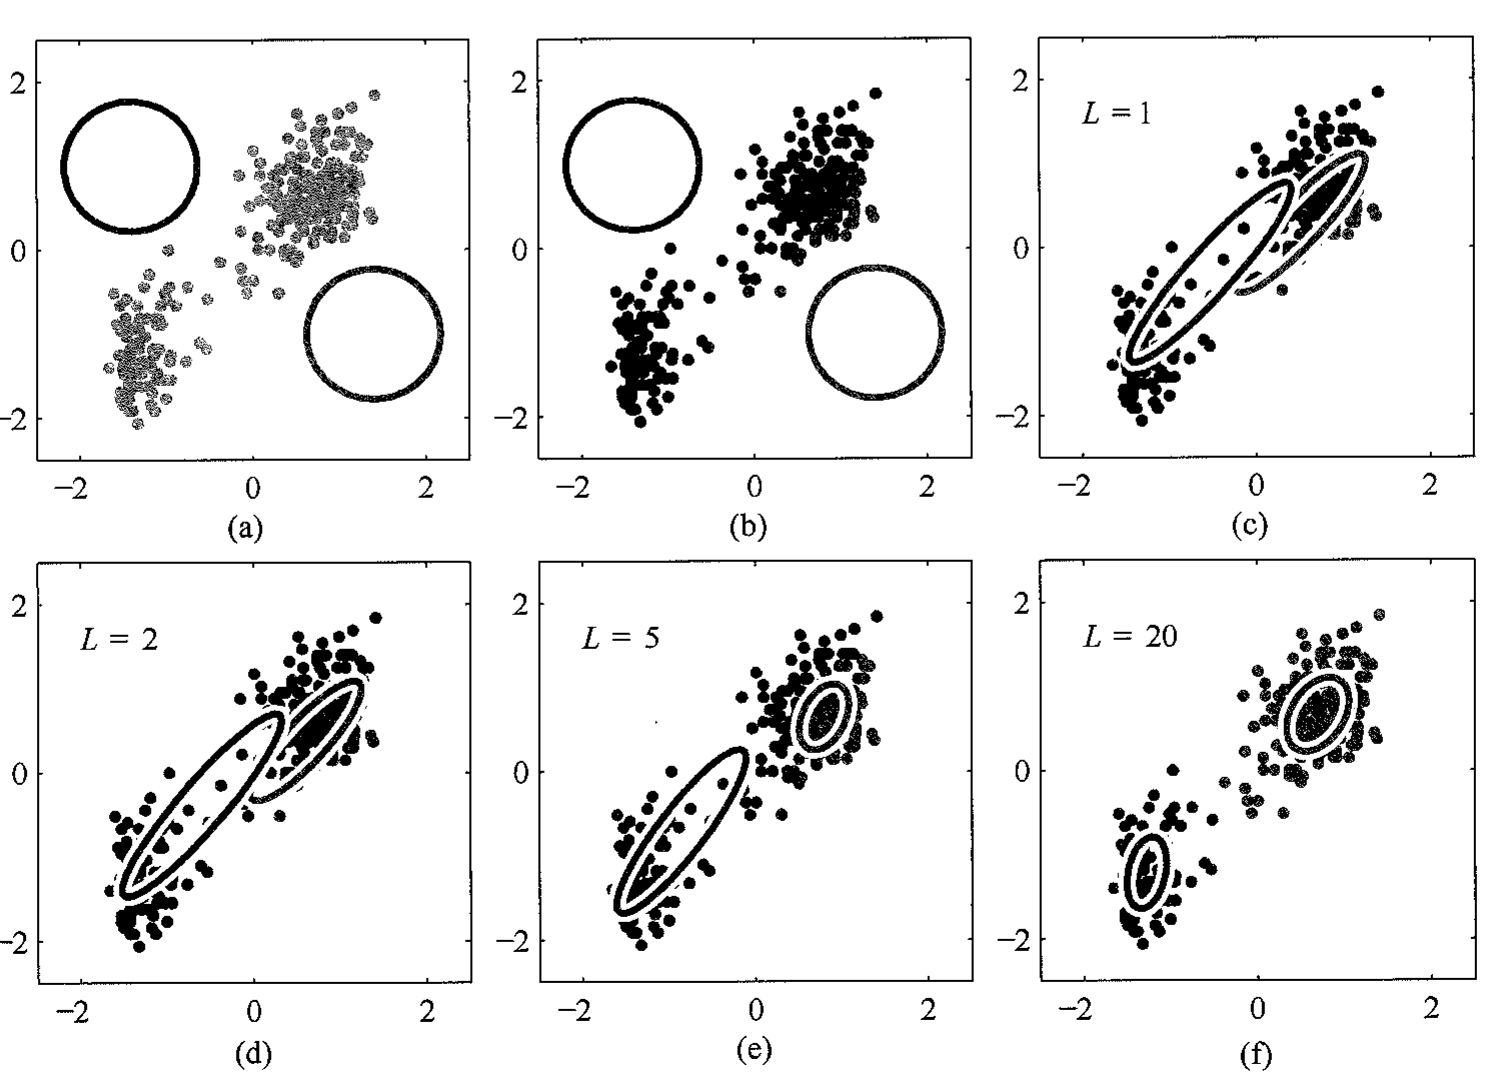
\includegraphics[width=0.92\textwidth]{ch15-fig15.7-em-iter.png}
\caption{将 EM 算法应用于老忠实喷泉数据集，该数据集在\cref{figure:ch15-kmeans}中用于说明 K 均值算法}
\label{figure:ch15-em-iter}
\end{figure}

\begin{remark}（重构新增）
\cref{figure:ch15-em-iter}中每个分图左上角的 $L$ 表示已经完成的完整 EM 循环次数，而每个分量画出的两条轮廓线分别是一倍标准差与两倍标准差的等密度线。由于参数是在 E 步骤之后、M 步骤之前被固定的，图中每一轮“颜色（责任）—轮廓（参数）”的交替正好对应\cref{proposition:ch15-GMM最大似然}中方程组的迭代求根：先按当前参数算责任，再按责任算参数。注意 (f) 中两个分量仍有部分重叠，这说明 EM 收敛到的是对数似然的一个局部极大点，而不是把两个簇完全分开的“理想”解；初值若选得更差，收敛结果可能完全不同（见本节末的讨论）。
\end{remark}

请注意，与 K 均值算法相比，EM 算法需要进行更多的迭代才能达到（近似）收敛，而且每个循环都需要进行更多的计算。因此，人们通常会运行 K 均值算法来找到 Gauss 混合模型的初始状态，随后使用 EM 算法进行调整。一种便捷的做法就是把协方差矩阵初始化为 K 均值算法以找到各个聚类的样本协方差，而混合系数可以设置为数据点被分配给相应聚类的比例。为了规避似然函数的奇异性——Gauss 分量坍缩至特定数据点的情况——我们必须采取诸如参数正则化的技术。需要强调的是，对数似然函数通常会有多个局部最大值，并且 EM 算法不能保证找到全局最大值。考虑到应用于 Gauss 混合模型的 EM 算法的重要性，我们在算法 15.2 中对它做了总结。

\begin{center}
\setlength{\fboxsep}{7pt}%
\fbox{\begin{minipage}{0.8\textwidth}
\centering\textbf{算法 15.2\quad 应用于 Gauss 混合模型的 EM 算法}\par
\vspace{5pt}
\begin{flushleft}
\textbf{Input:} 初始模型参数 $\{\bm{\mu}_k\},\{\bm{\Sigma}_k\},\{\pi_k\}$\\
\hspace*{1.5em}数据集 $\{\bm{x}_1,\cdots,\bm{x}_N\}$\\
\textbf{Output:} 最终模型参数 $\{\bm{\mu}_k\},\{\bm{\Sigma}_k\},\{\pi_k\}$\\
\textbf{repeat}\\
\hspace*{1.5em}// E 步骤\\
\hspace*{1.5em}\textbf{for} $n\in\{1,\cdots,N\}$ \textbf{do}\\
\hspace*{3em}\textbf{for} $k\in\{1,\cdots,K\}$ \textbf{do}\\
\hspace*{3em}$\gamma(z_{nk})\leftarrow\pi_k\mathcal{N}(\bm{x}_n\,|\,\bm{\mu}_k,\bm{\Sigma}_k)\big/\sum_{j=1}^{K}\pi_j\mathcal{N}(\bm{x}_n\,|\,\bm{\mu}_j,\bm{\Sigma}_j)$\\
\hspace*{3em}\textbf{end for}\\
\hspace*{1.5em}\textbf{end for}\\
\hspace*{1.5em}// M 步骤\\
\hspace*{1.5em}\textbf{for} $k\in\{1,\cdots,K\}$ \textbf{do}\\
\hspace*{3em}$N_k\leftarrow\sum_{n=1}^{N}\gamma(z_{nk})$\\
\hspace*{3em}$\bm{\mu}_k\leftarrow\dfrac{1}{N_k}\sum_{n=1}^{N}\gamma(z_{nk})\bm{x}_n$\\
\hspace*{3em}$\bm{\Sigma}_k\leftarrow\dfrac{1}{N_k}\sum_{n=1}^{N}\gamma(z_{nk})(\bm{x}_n-\bm{\mu}_k)(\bm{x}_n-\bm{\mu}_k)^{\mathsf T}$\\
\hspace*{3em}$\pi_k\leftarrow\dfrac{N_k}{N}$\\
\hspace*{1.5em}\textbf{end for}\\
\hspace*{1.5em}// 对数似然\\
\hspace*{1.5em}$\mathcal{L}\leftarrow\sum_{n=1}^{N}\ln\!\left\{\sum_{k=1}^{K}\pi_k\mathcal{N}(\bm{x}_n\,|\,\bm{\mu}_k,\bm{\Sigma}_k)\right\}$\\
\textbf{until} 收敛\\
\textbf{return} $\{\bm{\mu}_k\},\{\bm{\Sigma}_k\},\{\pi_k\}$
\end{flushleft}
\end{minipage}}
\end{center}

Gauss 混合模型非常灵活，如果模型参数选择得当，只需要给定足够数量的分量，就可以高精度地逼近复杂的数据分布。然而在实践中，尤其在高维空间中，分量的数量可能非常大。这个问题在\cref{figure:ch15-twomoons}中有所体现。尽管如此，Gauss 混合模型仍十分有用。此外，理解 Gauss 混合模型能为我们理解具有连续潜变量的模型和基于深度神经网络的生成式模型奠定基础，后者对高维空间的扩展性要好得多（参见\cref{chapter:ch16-连续潜变量}）。

\begin{figure}[htbp]
\centering
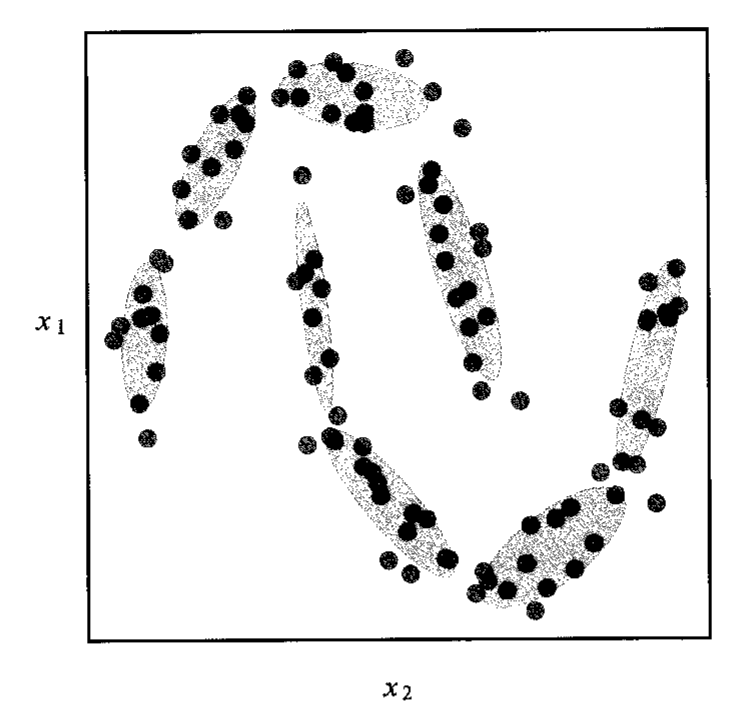
\includegraphics[width=0.42\textwidth]{ch15-fig15.8-twomoons-gmm.png}
\caption{拟合到“双月”数据集的 Gauss 混合模型，这表明可能需要大量的混合分量才能准确表示复杂的数据分布。这里椭圆表示对应混合分量的恒定密度等值线。随着我们进入更高维空间，精确建模分布所需的分量的数量可能会大到不可接受}
\label{figure:ch15-twomoons}
\end{figure}

\end{document}
